\documentclass[a4 paper]{article}
% Set target color model to RGB
\usepackage[inner=2.0cm,outer=2.0cm,top=2.5cm,bottom=2.5cm]{geometry}
\usepackage{setspace}
\usepackage[rgb]{xcolor}
\usepackage{verbatim}
\usepackage{subcaption}
\usepackage{amsgen,amsmath,amstext,amsbsy,amsopn,tikz,amssymb}
\usepackage{fancyhdr}
\usepackage[colorlinks=true, urlcolor=blue,  linkcolor=blue, citecolor=blue]{hyperref}
\usepackage[colorinlistoftodos]{todonotes}
\usepackage{rotating}
\usepackage{tikz}
\usetikzlibrary{decorations.pathreplacing} 
\usepackage{float}
\usepackage{minted}


%\usetikzlibrary{through,backgrounds}
\hypersetup{%
pdfauthor={Ashudeep Singh},%
pdftitle={Homework},%
pdfkeywords={Tikz,latex,bootstrap,uncertaintes},%
pdfcreator={PDFLaTeX},%
pdfproducer={PDFLaTeX},%
}
%\usetikzlibrary{shadows}
% \usepackage[francais]{babel}
\usepackage{booktabs}
\newcommand{\ra}[1]{\renewcommand{\arraystretch}{#1}}

\newtheorem{thm}{Theorem}[section]
\newtheorem{prop}[thm]{Proposition}
\newtheorem{lem}[thm]{Lemma}
\newtheorem{cor}[thm]{Corollary}
\newtheorem{defn}[thm]{Definition}
\newtheorem{rem}[thm]{Remark}
\numberwithin{equation}{section}

\newcommand{\homework}[6]{
   \pagestyle{myheadings}
   \thispagestyle{plain}
   \newpage
   \setcounter{page}{1}
   \noindent
   \begin{center}
   \framebox{
      \vbox{\vspace{2mm}
    \hbox to 6.28in { {\bf 67678 - Introduction to Control with Learning \hfill {\small (#2)}} }
       \vspace{6mm}
       \hbox to 6.28in { {\Large \hfill #1  \hfill} }
       \vspace{6mm}
       \hbox to 6.28in { {\it Instructor: {\rm #3} \hfill Name: {\rm #5} {\rm #6}} }
       %\hbox to 6.28in { {\it TA: #4  \hfill #6}}
      \vspace{2mm}}
   }
   \end{center}
   \markboth{#5 -- #1}{#5 -- #1}
   \vspace*{4mm}
}

\newcommand{\problempoints}[2]{~\\\fbox{\textbf{Problem #1}}\hfill (#2 points)\newline\newline}
\newcommand{\subproblem}[1]{~\newline\textbf{(#1)}}
\newcommand{\D}{\mathcal{D}}
\newcommand{\Hy}{\mathcal{H}}
\newcommand{\VS}{\textrm{VS}}
\newcommand{\solution}{~\newline\textbf{\textit{(Solution)}} }

\newcommand{\important}[1]{\textcolor{blue}{\textit{\textbf{#1}}}} 

\newcommand{\problem}[1]{~\\\fbox{\textbf{Problem #1}} \newline\newline}


\newcommand{\bbF}{\mathbb{F}}
\newcommand{\bbX}{\mathbb{X}}
\newcommand{\bI}{\mathbf{I}}
\newcommand{\bX}{\mathbf{X}}
\newcommand{\bY}{\mathbf{Y}}
\newcommand{\bepsilon}{\boldsymbol{\epsilon}}
\newcommand{\balpha}{\boldsymbol{\alpha}}
\newcommand{\bbeta}{\boldsymbol{\beta}}
\newcommand{\0}{\mathbf{0}}

\setlength{\parindent}{0pt}


\begin{document}
\homework{Assignment 1 - LQR Control}{Due: 02/06/24}{Oron Sabag}{}{Hadar Tal}{}
\textbf{Instructions}: 
\begin{itemize}
    \item The assignment is to be done individually.
    \item Submit your assignment as a single PDF file.
    \item Read all the Questions carefully before you start working on the assignment.
    \item This file contains \underbar{extra materials} for those who are interested in learning the tools used in the 
        assignment's solution. \underbar{Reading it is not required to complete the assignment.}
    \item You can use any python library to solve the problems.
\end{itemize}

% * * * * * * * * * * * * * * * * * * * * * * * * 
% * * * * * * * * * * * * * * * * * * * * * * * * 
% * * * * * * * * * * * * * * * * * * * * * * * * 
% * * * * * * * * * * * * * * * * * * * * * * * * 
% * * * * * * * * * * * * * * * * * * * * * * * * 
% * * * * * * * * * * * * * * * * * * * * * * * * 
% * * * * * * * * * * * * * * * * * * * * * * * * 
% * * * * * * * * * * * * * * * * * * * * * * * * 
% * * * * * * * * * * * * * * * * * * * * * * * * 
% * * * * * * * * * * * * * * * * * * * * * * * * 
% * * * * * * * * * * * * * * * * * * * * * * * * 
% * * * * * * * * * * * * * * * * * * * * * * * * 
% * * * * * * * * * * * * * * * * * * * * * * * * 
% * * * * * * * * * * * * * * * * * * * * * * * * 
% * * * * * * * * * * * * * * * * * * * * * * * * 
% * * * * * * * * * * * * * * * * * * * * * * * * 
\section{Continuous-time System}

In the lecture, we focused on discrete linear systems. However, real-world systems often operate in continuous time, 
making it essential to understand the transition to continuous-time systems and the associated control strategies.

\subsection{Motivation for Continuous-time Systems}
Continuous-time systems are ubiquitous in engineering and natural processes. Examples include electrical circuits, 
mechanical systems, and biological systems. Unlike discrete systems, which are defined at specific time intervals, 
continuous systems evolve over time according to differential equations. This continuous evolution provides a more 
accurate representation of physical phenomena, allowing for precise modeling and control.

\subsection{Equations of the Dynamics}
The state-space representation of a continuous-time linear system is given by the following set of differential equations:

\begin{equation}
    \dot{x}(t) = A x(t) + B u(t)
\end{equation}

where:
\begin{itemize}
    \item $x(t) \in \mathbb{R}^n$ is the state vector.
    \item $u(t) \in \mathbb{R}^m$ is the control input.
    \item $A \in \mathbb{R}^{n \times n}$ is the state matrix.
    \item $B \in \mathbb{R}^{n \times m}$ is the input matrix.
\end{itemize}

\subsection{Linear Quadratic Regulator (LQR) Problem}
The LQR problem for continuous-time systems involves finding a control law that minimizes a quadratic cost function. 
The objective is to regulate the state of the system to the origin while minimizing the control effort. The cost function is defined as:

\begin{equation} \label{eq:continuous_cost_function}
    J(t) = \int_{0}^{t} \left( x(\tau)^T Q x(\tau) + u(\tau)^T R u(\tau) \right) d\tau
\end{equation}
where $Q \in \mathbb{R}^{n \times n}$ and $R \in \mathbb{R}^{m \times m}$ determine the relative importance of the state and 
control effort in the cost function.


\subsection{Comparison to Discrete-time LQR}
In discrete-time systems, the state-space representation is defined by difference equations rather than differential equations. 
The discrete-time LQR problem is similar to its continuous-time counterpart but with a cost function summed over discrete time steps. 
The key equations are:

\begin{equation}
    x_{k+1} = A_d x_k + B_d u_k, \quad k = 0, 1, 2, \ldots
\end{equation}
\begin{equation}
    J_N(u^N) = \sum_{k=0}^{N} \left( x_k^T Q x_k + u_k^T R u_k \right) + x_{N+1}^T Q_f x_{N+1}
\end{equation}
\begin{equation}
    u_k = -K_d x_k,
\end{equation}
where $K_d$ is the optimal control gain matrix.


\subsection{The Optimal Control}
In the lecture, we discussed the determination of the control gain matrix \( K \) for discrete-time systems using an iterative approach. 
This method involved solving a finite-horizon cost function through backward iteration, essentially using dynamic programming techniques. 
However, for continuous-time systems, the process leverages the \important{Continuous Algebraic Riccati equation} for an infinite-horizon cost function, 
providing a more direct and analytical solution (\ref{sec:riccati}).





% * * * * * * * * * * * * * * * * * * * * * * * * 
% * * * * * * * * * * * * * * * * * * * * * * * * 
% * * * * * * * * * * * * * * * * * * * * * * * * 
% * * * * * * * * * * * * * * * * * * * * * * * * 
% * * * * * * * * * * * * * * * * * * * * * * * * 
% * * * * * * * * * * * * * * * * * * * * * * * * 
% * * * * * * * * * * * * * * * * * * * * * * * * 
% * * * * * * * * * * * * * * * * * * * * * * * * 
% * * * * * * * * * * * * * * * * * * * * * * * * 
% * * * * * * * * * * * * * * * * * * * * * * * * 
% * * * * * * * * * * * * * * * * * * * * * * * * 
% * * * * * * * * * * * * * * * * * * * * * * * * 
% * * * * * * * * * * * * * * * * * * * * * * * * 
% * * * * * * * * * * * * * * * * * * * * * * * * 
% * * * * * * * * * * * * * * * * * * * * * * * * 
% * * * * * * * * * * * * * * * * * * * * * * * * 
\section{Inverted Pendulum on a Cart}


The inverted pendulum on a cart is a classic problem in control theory and dynamics, often used to illustrate and test various control strategies. 
The system consists of a pendulum attached to a cart that can move horizontally. 
The goal is to design a controller that can stabilize the pendulum at the top position while regulating the position of the cart.

\subsection{Formulation of the Problem}

\begin{figure}[H]
    \centering
    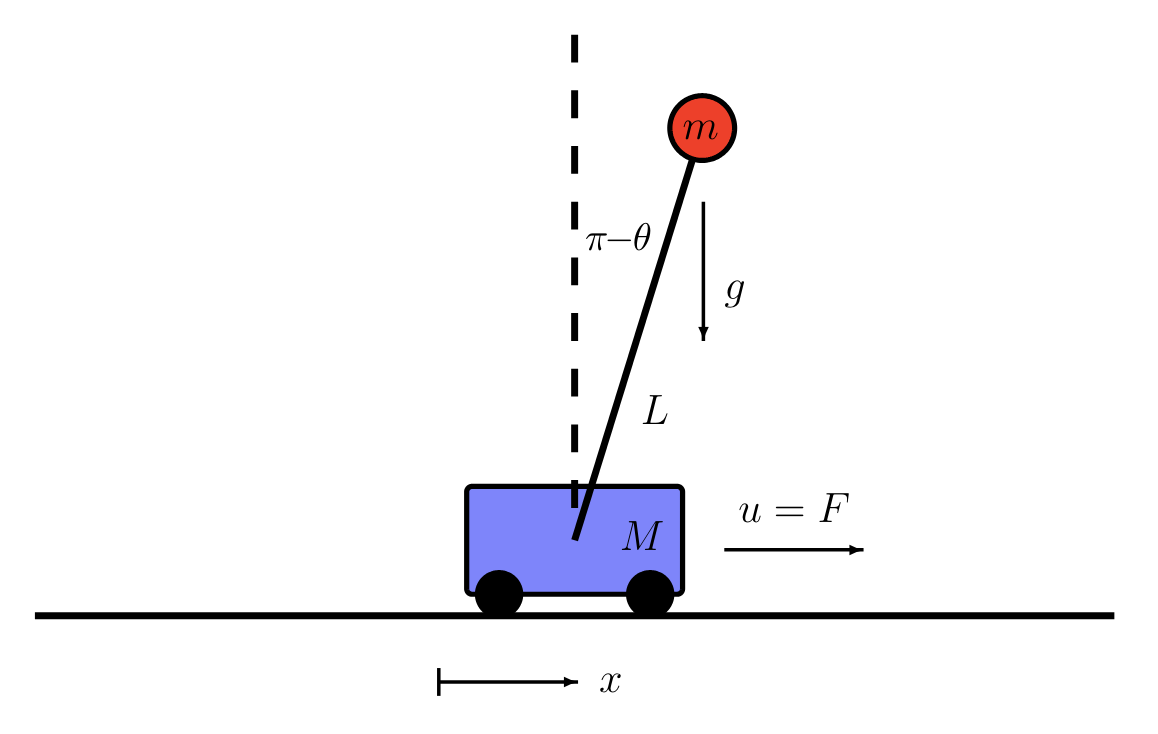
\includegraphics[width=0.6\textwidth]{./figs/inverted_pendulum_on_a_cart.png}
    \caption{Schematic of inverted pendulum on a cart.}
\end{figure}


The dynamics of the system can be described by the following set of nonlinear differential equations:
\begin{align}
    \dot{x} &= v \label{eq:cart_position} \\
    \ddot{x} &= \frac{-m^2 L^2 g \cos(\theta) \sin(\theta) + m L^2 \left( m L \omega^2 \sin(\theta) - \delta v \right) + m L^2 u}{m L^2 \left( M + m (1 - \cos(\theta)^2) \right)} \label{eq:cart_velocity} \\
    \dot{\theta} &= \omega \label{eq:pendulum_angle} \\
    \ddot{\theta} &= \frac{(m + M) m g L \sin(\theta) - m L \cos(\theta) \left( m L \omega^2 \sin(\theta) - \delta v \right) + m L \cos(\theta) u}{m L^2 \left( M + m (1 - \cos(\theta)^2) \right)} \label{eq:pendulum_angular_velocity}
\end{align}
where \( x \) is the cart position, \( v \) is the velocity, \( \theta \) is the pendulum angle, \( \omega \) is the angular velocity, \( m \) is the pendulum mass, \( M \) is the cart mass, \( L \) is the pendulum arm length, \( g \) is the gravitational acceleration, \( \delta \) is a friction damping on the cart, and \( u \) is a control force applied to the cart.


\problem{1 - Modeling the Inverted Pendulum System}

\textcolor{purple}{
\subproblem{a} Implement the function \texttt{dynamics} in the provided Python file \texttt{inverted\_pendulum.py}.
}

\begin{minted}[fontsize=\footnotesize]{python}
    def dynamics(y, m, M, L, g, delta, u):
        """
        Compute the state derivative.
        :param y: state vector
        :param m: pendulum mass
        :param M: cart mass
        :param L: pendulum length
        :param g: gravitational acceleration
        :param delta: friction damping
        :param u: control input
        :return dy: state derivative
        """
\end{minted}

\medbreak

\textcolor{teal}{
    Solution:
}

\begin{minted}[fontsize=\footnotesize]{python}
    def dynamics(y, m, M, L, g, delta, u):
        """
        Compute the state derivatives.
        :param y: state vector
        :param m: pendulum mass
        :param M: cart mass
        :param L: pendulum length
        :param g: gravitational acceleration
        :param delta: friction damping
        :param u: control input
        :return: dy: state derivative
        """
        theta = y[2]
        theta_dot = y[3]
        sin_theta = np.sin(theta)
        cos_theta = np.cos(theta)
        D = m * (L ** 2) * (M + m * (1 - cos_theta ** 2))    
        dy = np.array([
            y[1],
            (1 / D) * (
                -(m ** 2) * (L ** 2) * g * cos_theta * sin_theta 
                + m * (L ** 2) * (m * L * (theta_dot ** 2) * sin_theta - delta * y[1])
            ) + m * (L ** 2) * (1 / D) * u,
            y[3],
            (1 / D) * (
                (m + M) * m * g * L * sin_theta 
                - m * L * cos_theta * (m * L * (theta_dot ** 2) * sin_theta 
                - delta * y[1])
            ) - m * L * cos_theta * (1 / D) * u
        ])
        return dy
\end{minted}


\medbreak

\textcolor{purple}{
    \subproblem{b} Are there exist matrices $A$ and $B$ such that $\forall t \in \mathbb{R}_{\geq 0}$,  $\dot{\mathbf{y_t}} = A \mathbf{y_t} + B u_t $? Justify your answer.
}

\medbreak

\textcolor{teal}{
    The system dynamics are nonlinear, as shown in equations \ref{eq:cart_position} - \ref{eq:pendulum_angular_velocity}. 
    Therefore, there are no matrices \( A \) and \( B \) that can linearize the system dynamics at all time points. 
    Linearization is only possible around specific operating points, such as the upright position of the pendulum. 
}

\medbreak

\textcolor{purple}{
    \subproblem{c} Linearize the system dynamics around the upright position (\(\theta = \pi\)) to obtain the linearized state-space representation:
    \begin{equation*}
        \dot{\mathbf{x}} = A \mathbf{x} + B u
    \end{equation*}
    where \( A \) and \( B \) are the state and input matrices, respectively. 
}

\medbreak

\textcolor{teal}{
    The linearized system dynamics around the upright position (\(\theta = \pi\)) are given by:
    \begin{equation*}
        \dot{\mathbf{y}} = \begin{bmatrix}
            0 & 1 & 0 & 0 \\
            0 & -\frac{\delta}{M} & \frac{m g}{M} & 0 \\
            0 & 0 & 0 & 1 \\
            0 & -\frac{\delta}{M L} & - \frac{(M + m) g}{M L} & 0
        \end{bmatrix} \mathbf{y} + 
        \begin{bmatrix}
            0 \\
            \frac{1}{M} \\
            0 \\
            \frac{1}{M L}
        \end{bmatrix} u
    \end{equation*}
}

\bigbreak

\textcolor{purple}{
    \subproblem{d} Implement the following functions.
}

\begin{minted}[fontsize=\footnotesize]{python}
    def get_a_matrix(m, M, L, g, delta):
        """
        :return A: state matrix
        """

    def get_b_matrix(m, M, L, g, delta):
        """
        :return B: input matrix
        """
\end{minted}

\medbreak

\textcolor{teal}{
    Solution:
}

\begin{minted}[fontsize=\footnotesize]{python}
    def get_a_matrix(m, M, L, g, delta):
        """
        :return A: state matrix
        """
        A = np.array([
            [0, 1, 0, 0],
            [0, -delta / M, m * g / M, 0],
            [0, 0, 0, 1],
            [0, -delta / (M * L), - (M + m) * g / (M * L), 0]
        ])
        return A

    def get_b_matrix(m, M, L, g, delta):
        """
        :return B: input matrix
        """
        B = np.array([
            [0],
            [1 / M],
            [0],
            [1 / (M * L)]
        ])
        return B
\end{minted}


\problem{2 - LQR Control for the Inverted Pendulum System}

We will set the following parameters for the inverted pendulum system:
\begin{itemize}
    \item Pendulum mass: \( m = 0.1 \) kg
    \item Cart mass: \( M = 1.0 \) kg
    \item Pendulum length: \( L = 0.5 \) m
    \item Gravitational acceleration: \( g = 9.81 \) m/s\(^2\)
    \item Friction damping: \( \delta = 0.1 \) Ns/m
\end{itemize}

\textcolor{purple}{
    \subproblem{a} Calculate and print the State feedback gain matrix \( K \) for the LQR controller (bonus points for using the continuous-time Riccati equation).
}

\medbreak

\textcolor{teal}{
    Solution:
}

\begin{minted}[fontsize=\footnotesize]{python}
    K, S, E = control.lqr(A, B, Q, R)
\end{minted}

\bigbreak



    


\bigbreak
\bigbreak
\bigbreak
\bigbreak
\bigbreak
















% * * * * * * * * * * * * * * * * * * * * * * * * 
% * * * * * * * * * * * * * * * * * * * * * * * * 
% * * * * * * * * * * * * * * * * * * * * * * * * 
% * * * * * * * * * * * * * * * * * * * * * * * * 
% * * * * * * * * * * * * * * * * * * * * * * * * 
% * * * * * * * * * * * * * * * * * * * * * * * * 
% * * * * * * * * * * * * * * * * * * * * * * * * 
% * * * * * * * * * * * * * * * * * * * * * * * * 
% * * * * * * * * * * * * * * * * * * * * * * * * 
% * * * * * * * * * * * * * * * * * * * * * * * * 
% * * * * * * * * * * * * * * * * * * * * * * * * 
% * * * * * * * * * * * * * * * * * * * * * * * * 
% * * * * * * * * * * * * * * * * * * * * * * * * 
% * * * * * * * * * * * * * * * * * * * * * * * * 
% * * * * * * * * * * * * * * * * * * * * * * * * 
% * * * * * * * * * * * * * * * * * * * * * * * * 
\newpage
\textbf{\huge{Extra material}}
\section{Riccati Equation}\label{sec:riccati}

This derivation of Riccati equation will provide an example of how to solve convex optimization problems using the \important{calculus of variations}, 
and it will also provide a template for computing the optimal control solution for nonlinear systems. 

First, we will add a terminal cost to our LQR cost function in \ref{eq:continuous_cost_function}, 
and also introduce a factor of 1/2 to simplify computations:
\begin{equation}
    J = \int_{0}^{t_f} \underbrace{\frac{1}{2} \left( x^T Q x + u^T R u \right)}_\text{Lagrangian $\mathcal{L}$} d\tau + 
        \underbrace{\frac{1}{2} x(t_f)^T Q_f x(t_f)}_\text{Terminal cost}
\label{eq:cost_function}
\end{equation}
The goal is to minimize the quadratic cost function \( J \) subject to the dynamical constraint:
\begin{equation}
    \dot{x} = A x + B u.
\label{eq:dynamic_constraint}
\end{equation}
We may solve this using the calculus of variations by introducing the following augmented cost function:
\begin{equation}
    J_{aug} = \int_{0}^{t_f} \left[ \frac{1}{2} \left( x^T Q x + u^T R u \right) + \lambda^T (A x + B u - \dot{x}) \right] 
    dt + \frac{1}{2} x(t_f)^T Q_f x(t_f)
\label{eq:augmented_cost_function}
\end{equation}
The variable \( \lambda \) is a \important{Lagrange multiplier}, called the co-state, that enforces the dynamic constraints. \( \lambda \) may 
take any value and \( J_{aug} = J \) will hold.

\bigbreak

Taking the total variation of \( J_{aug} \) in \ref{eq:augmented_cost_function} yields:
\begin{equation}
    \delta J_{aug} = \int_{0}^{t_f} \left[ \frac{\partial \mathcal{L}}{\partial x} \delta x + \frac{\partial \mathcal{L}}{\partial u} \delta u 
        + \lambda^T A \delta x + \lambda^T B \delta u - \lambda^T \delta \dot{x} \right] dt + Q_f x(t_f) \delta x(t_f)
\label{eq:total_variation}
\end{equation}
The partial derivatives of the Lagrangian are \( \frac{\partial \mathcal{L}}{\partial x} = x^T Q \) and 
\( \frac{\partial \mathcal{L}}{\partial u} = u^T R \). The last term in the integral may be modified using integration by parts:

\begin{equation}
    -\int_{0}^{t_f} \lambda^T \delta \dot{x} dt = -\lambda^T (t_f) \delta x(t_f) + \lambda^T (0) \delta x(0) + 
    \int_{0}^{t_f} \dot{\lambda}^T \delta x dt.
\label{eq:integration_by_parts}
\end{equation}
The term \( \lambda^T (0) \delta x(0) \) is equal to zero, or else the control system would be non-causal 
(i.e., then future control could change the initial condition of the system).

\bigbreak

Finally, the total variation of the augmented cost function in \ref{eq:total_variation} simplifies as follows:
\begin{equation}
    \delta J_{aug} = \int_{0}^{t_f} \left[ x^T Q + \lambda^T A + \dot{\lambda}^T \right] \delta x dt + 
    \int_{0}^{t_f} \left[ u^T R + \lambda^T B \right] \delta u dt + (x(t_f)^T Q_f - \lambda^T (t_f)) \delta x(t_f).
\label{eq:simplified_total_variation}
\end{equation}
\textbf{Each variation term in \ref{eq:simplified_total_variation} must equal zero for an optimal control solution that minimizes \( J \).} 
Thus, we may break this up into three equations:
\begin{equation}
    x^T Q + \lambda^T A + \dot{\lambda}^T = 0
\label{eq:variation_term_1}
\end{equation}
\begin{equation}
    u^T R + \lambda^T B = 0
\label{eq:variation_term_2}
\end{equation}
\begin{equation}
    x(t_f)^T Q_f - \lambda^T (t_f) = 0. 
\label{eq:variation_term_3}
\end{equation}
Note that the constraint in \ref{eq:variation_term_3} represents an initial condition for the reverse-time equation for 
\( \lambda \) starting at \( t_f \). Thus, the dynamics in \ref{eq:dynamic_constraint} with initial condition \( x(0) = x_0 \) 
and \ref{eq:variation_term_3} with the final-time condition \( \lambda (t_f) = Q_f x(t_f) \) form a two-point boundary value problem. 
This may be integrated numerically to find the optimal control solution, even for nonlinear systems.

\bigbreak

Because the dynamics are linear, it is possible to posit the form \( \lambda = P x \), and substitute into \ref{eq:variation_term_1} above. 
The first equation becomes:
\begin{equation}
    \left( \dot{P} x + P \dot{x} \right)^T + x^T Q + \lambda^T A = 0.
\label{eq:posit_form}
\end{equation}
Taking the transpose, and substituting \ref{eq:dynamic_constraint} in for \( \dot{x} \), yields:
\begin{equation}
    \dot{P} x + P (A x + B u) + Q x + A^T P x = 0.
\label{eq:transpose_substitution}
\end{equation}
From \ref{eq:variation_term_2}, we have
\begin{equation}
    u = -R^{-1} B^T \lambda = -R^{-1} B^T P x.
\label{eq:control_input}
\end{equation}
Finally, combining yields:
\begin{equation}
    \dot{P} x + P A x + A^T P x - P B R^{-1} B^T P x + Q x = 0.
\label{eq:combining_yields}
\end{equation}
This equation must be true for all \( x \), and so it may also be written as a matrix equation.
 Dropping the terminal cost and letting time go to infinity, the \( \dot{P} \) term disappears, and we recover the
\important{Continuous Algebraic Riccati equation (CARE) }:
\begin{equation}
    P A + A^T P - P B R^{-1} B^T P + Q = 0.
\label{eq:riccati_equation}
\end{equation}
Although this procedure is somewhat involved, each step is relatively straightforward. In addition, the dynamics in \ref{eq:dynamic_constraint} 
may be replaced with nonlinear dynamics \( \dot{x} = f(x,u) \), and a similar nonlinear two-point boundary value problem may be formulated 
with \( \frac{\partial f}{\partial x} \) replacing \( A \) and \( \frac{\partial f}{\partial u} \) replacing \( B \). 
This procedure is extremely general, and may be used to numerically obtain nonlinear optimal control trajectories.


% * * * * * * * * * * * * * * * * * * * * * * * * 
% * * * * * * * * * * * * * * * * * * * * * * * * 
% * * * * * * * * * * * * * * * * * * * * * * * * 
% * * * * * * * * * * * * * * * * * * * * * * * * 
% * * * * * * * * * * * * * * * * * * * * * * * * 
% * * * * * * * * * * * * * * * * * * * * * * * * 
% * * * * * * * * * * * * * * * * * * * * * * * * 
% * * * * * * * * * * * * * * * * * * * * * * * * 
% * * * * * * * * * * * * * * * * * * * * * * * * 
% * * * * * * * * * * * * * * * * * * * * * * * * 
% * * * * * * * * * * * * * * * * * * * * * * * * 
% * * * * * * * * * * * * * * * * * * * * * * * * 
% * * * * * * * * * * * * * * * * * * * * * * * * 
% * * * * * * * * * * * * * * * * * * * * * * * * 
% * * * * * * * * * * * * * * * * * * * * * * * * 
% * * * * * * * * * * * * * * * * * * * * * * * * 
\newpage
\section{Euler-Lagrange Equations}


% * * * * * * * * * * * * * * * * * * * * * * * * 
% * * * * * * * * * * * * * * * * * * * * * * * * 
% * * * * * * * * * * * * * * * * * * * * * * * * 
% * * * * * * * * * * * * * * * * * * * * * * * * 
% * * * * * * * * * * * * * * * * * * * * * * * * 
% * * * * * * * * * * * * * * * * * * * * * * * * 
% * * * * * * * * * * * * * * * * * * * * * * * * 
% * * * * * * * * * * * * * * * * * * * * * * * * 
% * * * * * * * * * * * * * * * * * * * * * * * * 
% * * * * * * * * * * * * * * * * * * * * * * * * 
% * * * * * * * * * * * * * * * * * * * * * * * * 
% * * * * * * * * * * * * * * * * * * * * * * * * 
% * * * * * * * * * * * * * * * * * * * * * * * * 
% * * * * * * * * * * * * * * * * * * * * * * * * 
% * * * * * * * * * * * * * * * * * * * * * * * * 
% * * * * * * * * * * * * * * * * * * * * * * * * 
\newpage
\section{Euler-Lagrange Equations}




% * * * * * * * * * * * * * * * * * * * * * * * * 
% * * * * * * * * * * * * * * * * * * * * * * * * 
% * * * * * * * * * * * * * * * * * * * * * * * * 
% * * * * * * * * * * * * * * * * * * * * * * * * 
% * * * * * * * * * * * * * * * * * * * * * * * * 
% * * * * * * * * * * * * * * * * * * * * * * * * 
% * * * * * * * * * * * * * * * * * * * * * * * * 
% * * * * * * * * * * * * * * * * * * * * * * * * 
% * * * * * * * * * * * * * * * * * * * * * * * * 
% * * * * * * * * * * * * * * * * * * * * * * * * 
% * * * * * * * * * * * * * * * * * * * * * * * * 
% * * * * * * * * * * * * * * * * * * * * * * * * 
% * * * * * * * * * * * * * * * * * * * * * * * * 
% * * * * * * * * * * * * * * * * * * * * * * * * 
% * * * * * * * * * * * * * * * * * * * * * * * * 
% * * * * * * * * * * * * * * * * * * * * * * * * 
\newpage
\begin{thebibliography}{9}

    \bibitem{brunton2019}
    S. Brunton, and J. Kutz,
    \textit{Data-Driven Science and Engineering: Machine Learning, Dynamical Systems, and Control}.
    Cambridge: Cambridge University Press, 2019.
    doi:10.1017/9781108380690
    
    \bibitem{brunton2017}
    S. Brunton,
    \textit{Linear Quadratic Regulator (LQR) Control for the Inverted Pendulum on a Cart [Control Bootcamp]}, 2017.
    
\end{thebibliography}

\end{document} 
